\documentclass[10pt,letterpaper]{article}
\usepackage[margin=0.65in]{geometry}
\usepackage[T1]{fontenc}
\usepackage{lmodern,booktabs,amsmath,microtype,xcolor,graphicx}
\usepackage[hidelinks]{hyperref}
\pagestyle{empty}
\setlength{\parindent}{0pt}
\setlength{\parskip}{5pt}
\begin{document}
{\Large\bfseries Exp 1: Ten Provers (Lean)}\hfill {\small 26 September 2026}
\vspace{2pt}\hrule
\textbf{Result.} At 480 reviews, weights exceeded context by 0.132 score units (95\% CI [0.053, 0.227]). The first observed lead that persisted through the remaining checkpoints was at 120 reviews.

\textbf{Design.} Ten Qwen3-8B workers per arm attempted small Lean list lemmas
with at most three compiler calls. The no-feedback, context, and LoRA arms each
ran 480 sessions over 4 rounds. DeepSeek-V3.1 reviewed
1440 reports. Context and weights received the same cumulative
no-feedback-arm reviews: context retrieved whole examples within 8,000 tokens;
rank-16 LoRA was retrained from base, with loss only on corrected final reports.
The scorer never supplied training targets or reward.

\textbf{Reporting accuracy.} Frozen base-agent trajectories were generated once
for 40 held-out lemmas (120 traces). Each checkpoint produced five reports per
trace at temperature 0.7. Score $F=P\times R$ measures precision and recall of
the structured status/event header; prose is unscored. Malformed reports score zero. The paired 95\%
interval resamples 20 lemma families (10,000 draws).

\begin{minipage}[t]{0.58\linewidth}
\vspace{0pt}
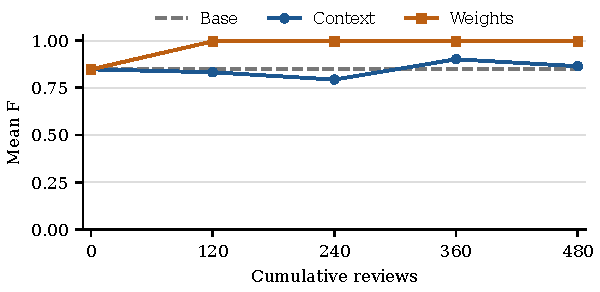
\includegraphics[width=\linewidth]{results-curve.pdf}
\end{minipage}\hfill
\begin{minipage}[t]{0.39\linewidth}
\vspace{3pt}\centering\small
\begin{tabular}{rccc}
\toprule
Reviews & Base & Context & Weights\\
\midrule
0 & 0.848 & 0.848 & 0.848 \\
120 & 0.848 & 0.832 & 0.996 \\
240 & 0.848 & 0.793 & 0.996 \\
360 & 0.848 & 0.901 & 0.996 \\
480 & 0.848 & 0.864 & 0.996 \\
\bottomrule
\end{tabular}
\par\raggedright\footnotesize
Optimizer steps: 32, 45, 69, 90.
Always reporting compile failure: $F=0.942$ (selected on corrected training reports).
\end{minipage}

\textbf{Does Sun help the analyst?} A fresh DeepSeek-V3.1 analyst inspected
the same 120 sessions through transcripts (T), transcripts plus ordinary
Git history (T+), or transcripts plus Sun log/show/blame (S), with 15 calls per
episode and no access to earlier reviews or scorer verdicts. Sun recall was 0.583 versus 0.792 for transcripts, with similarly low precision. The primary E3/E6 comparison (overwrites or borrowed \texttt{sorry}) had only 1 inconsistency and is underpowered.
\begin{center}\small
\begin{tabular}{lrrrr}
\toprule
View & Precision & Recall & Specificity & E3/E6 recall\\
\midrule
Transcripts & 0.211 & 0.792 & 0.451 & 0.000 \\
Transcripts + Git & 0.230 & 0.667 & 0.683 & 0.000 \\
Transcripts + Sun & 0.220 & 0.583 & 0.622 & 0.000 \\
\bottomrule
\end{tabular}
\end{center}
{\footnotesize Budget-exhausted analyst episodes (T/T+/S): 0/0/2; scored as no flags.}

\textbf{Checks and limits.} Reviewer-corrected reports exactly matched the scorer in 90.6\% of sessions; 0 reviews failed.
All 160 reference proofs passed Lean and the clean-context check; six automated
scorer tests cover failures, statement changes, custom axioms, direct/transitive
\texttt{sorry}, omissions, and overwrite attribution. The planned human smoke test has not been completed.
This is one live run with one LoRA seed per checkpoint. Parameterized lemma
families overlap across splits, and no self-label or shuffled-label training
controls were run. Logged operational amendments repaired pagination, context
overflow, transport retries, and run snapshots. These results measure reporting on base-agent traces, not
general theorem-proving ability or deliberate deception.

{\footnotesize\textbf{Reproducibility.} Sun was initialized for the experiment,
run, pilot, held-out and arm repositories. Saved compiler receipts, Sun commits,
review checks, samples, source hashes, and exported adapters support offline
recomputation. Including pilots, saved successful calls imply an uncached token cost of \$78.92; reservations total \$117.26, excluding storage. Neither is a provider invoice.\quad Run: \texttt{20260926-01}.}
\end{document}
